% !TeX program = xelatex
% !TeX encoding = UTF-8
\documentclass[12pt,openany,oneside]{book}

% -----------------------------------------------------------------------------
% Page, mathematics, tables, graphics
% -----------------------------------------------------------------------------
\usepackage[a4paper,top=23mm,bottom=25mm,left=25mm,right=25mm,headheight=17pt]{geometry}
\usepackage{amsmath,amssymb,amsfonts,mathtools,bm}
\usepackage{amsthm}
\usepackage{booktabs,longtable,array,multirow,tabularx}
\usepackage{graphicx}
\graphicspath{{figures/}}
\usepackage{xcolor}
\usepackage{tikz}
\usetikzlibrary{arrows.meta,positioning,calc,fit,shapes.geometric,decorations.pathreplacing,matrix,patterns}
\usepackage[most]{tcolorbox}
\usepackage{enumitem}
\usepackage{listings}
\usepackage{caption}
\usepackage{subcaption}
\usepackage{float}
\usepackage{fancyhdr}
\usepackage{titlesec}
\usepackage{setspace}
\usepackage{microtype}
\usepackage{hyperref}
\usepackage{xepersian}

% -----------------------------------------------------------------------------
% Robust font configuration: same visual convention as Chapters 2 and 3,
% with automatic fallbacks to avoid missing-font failures.
% -----------------------------------------------------------------------------
\IfFontExistsTF{Amiri}
  {\settextfont[Scale=1.08]{Amiri}\setdigitfont{Amiri}}
  {\settextfont[Scale=1.05]{Noto Naskh Arabic}\setdigitfont{Noto Naskh Arabic}}
\IfFontExistsTF{DejaVu Serif}
  {\setlatintextfont{DejaVu Serif}}
  {\setlatintextfont{Latin Modern Roman}}
\IfFontExistsTF{DejaVu Sans Mono}
  {\setmonofont{DejaVu Sans Mono}}
  {\setmonofont{Latin Modern Mono}}

% -----------------------------------------------------------------------------
% Visual identity, matching the previous chapters
% -----------------------------------------------------------------------------
\definecolor{DeepBlue}{HTML}{163A5F}
\definecolor{Accent}{HTML}{B34B35}
\definecolor{SoftBlue}{HTML}{EAF2F8}
\definecolor{SoftGold}{HTML}{FFF6DF}
\definecolor{SoftGreen}{HTML}{EAF7EF}
\definecolor{SoftRed}{HTML}{FCEDEC}
\definecolor{SoftGray}{HTML}{F4F5F6}
\definecolor{CodeGray}{HTML}{F7F7F7}

\hypersetup{
  colorlinks=true,
  linkcolor=DeepBlue,
  citecolor=Accent,
  urlcolor=Accent,
  pdftitle={پردازش تصویر در دهه آینده ـ فصل چهارم: تصویر تصادفی و مدل‌های نویز},
  pdfauthor={جزوه درس کارشناسی ارشد}
}

\setstretch{1.22}
\setlength{\parskip}{0.35em}
\setlength{\parindent}{1.3em}
\setlist[itemize]{itemsep=0.25em,topsep=0.35em,leftmargin=9mm}
\setlist[enumerate]{itemsep=0.25em,topsep=0.35em,leftmargin=10mm}

\pagestyle{fancy}
\fancyhf{}
\fancyhead[R]{\small\thepage}
\fancyhead[L]{\small\nouppercase{\leftmark}}
\renewcommand{\headrulewidth}{0.4pt}

\titleformat{\chapter}[display]
  {\normalfont\huge\bfseries\color{DeepBlue}}
  {\filleft\Large فصل \thechapter}
  {8pt}
  {\filright}
\titleformat{\section}{\Large\bfseries\color{DeepBlue}}{\thesection}{0.7em}{}
\titleformat{\subsection}{\large\bfseries\color{Accent}}{\thesubsection}{0.7em}{}
\titleformat{\subsubsection}{\normalsize\bfseries\color{DeepBlue}}{\thesubsubsection}{0.7em}{}

% -----------------------------------------------------------------------------
% Theorems and boxes
% -----------------------------------------------------------------------------
\newtheorem{definition}{تعریف}[chapter]
\newtheorem{theorem}{قضیه}[chapter]
\newtheorem{proposition}{گزاره}[chapter]
\newtheorem{lemma}{لم}[chapter]
\newtheorem{example}{مثال}[chapter]
\newtheorem{remark}{نکته}[chapter]
\newtheorem{corollary}{نتیجه}[chapter]
\renewcommand{\proofname}{اثبات}

\newtcolorbox{learningbox}{colback=SoftBlue,colframe=DeepBlue,title=اهداف یادگیری,fonttitle=\bfseries,breakable,enhanced}
\newtcolorbox{keybox}[1][]{colback=SoftGold,colframe=Accent,title={#1},fonttitle=\bfseries,breakable,enhanced}
\newtcolorbox{futurebox}{colback=SoftGreen,colframe=green!50!black,title=پل به دهه آینده,fonttitle=\bfseries,breakable,enhanced}
\newtcolorbox{warningbox}{colback=SoftRed,colframe=red!65!black,title=خطای رایج,fonttitle=\bfseries,breakable,enhanced}
\newtcolorbox{workshopbox}[1][]{colback=SoftGray,colframe=black!55,title={کارگاه کد و آزمایش: #1},fonttitle=\bfseries,breakable,enhanced}
\newtcolorbox{researchbox}[1][]{colback=white,colframe=purple!65!black,title={خواندن مقاله و استاندارد: #1},fonttitle=\bfseries,breakable,enhanced}
\newtcolorbox{videobox}{colback=white,colframe=DeepBlue,title=تقسیم پیشنهادی ویدئوهای ۱۵ دقیقه‌ای,fonttitle=\bfseries,breakable,enhanced}
\newtcolorbox{proofbox}[1][]{colback=white,colframe=DeepBlue!65,title={مسیر اثبات: #1},fonttitle=\bfseries,breakable,enhanced}
\newtcolorbox{codecontract}{colback=SoftBlue,colframe=Accent,title=قرارداد میان ریاضیات و کد,fonttitle=\bfseries,breakable,enhanced}
\newtcolorbox{summarybox}{colback=SoftBlue,colframe=DeepBlue,title=جمع‌بندی فصل,fonttitle=\bfseries,breakable,enhanced}

% -----------------------------------------------------------------------------
% Mathematical notation
% -----------------------------------------------------------------------------
\newcommand{\R}{\mathbb{R}}
\newcommand{\C}{\mathbb{C}}
\newcommand{\N}{\mathbb{N}}
\newcommand{\Z}{\mathbb{Z}}
\newcommand{\E}{\mathbb{E}}
\newcommand{\Var}{\operatorname{Var}}
\newcommand{\Cov}{\operatorname{Cov}}
\newcommand{\Corr}{\operatorname{Corr}}
\newcommand{\Prob}{\mathbb{P}}
\newcommand{\KL}{\operatorname{D}_{\mathrm{KL}}}
\newcommand{\norm}[1]{\left\lVert #1\right\rVert}
\newcommand{\abs}[1]{\left\lvert #1\right\rvert}
\newcommand{\inner}[2]{\left\langle #1,#2\right\rangle}
\newcommand{\trans}{^{\mathsf T}}
\newcommand{\herm}{^{\mathsf H}}
\newcommand{\vect}[1]{\bm{#1}}
\newcommand{\op}[1]{\mathcal{#1}}
\newcommand{\argmin}{\operatorname*{arg\,min}}
\newcommand{\argmax}{\operatorname*{arg\,max}}
\newcommand{\trace}{\operatorname{tr}}
\newcommand{\diag}{\operatorname{diag}}
\newcommand{\rank}{\operatorname{rank}}
\newcommand{\median}{\operatorname{median}}
\newcommand{\MAD}{\operatorname{MAD}}
\newcommand{\iid}{\overset{\mathrm{iid}}{\sim}}
\newcommand{\Normal}{\mathcal{N}}
\newcommand{\Poisson}{\operatorname{Poisson}}
\newcommand{\GammaD}{\operatorname{Gamma}}
\newcommand{\Bernoulli}{\operatorname{Bernoulli}}
\newcommand{\Fisher}{\mathcal{I}}
\newcommand{\MSE}{\operatorname{MSE}}
\newcommand{\AIC}{\operatorname{AIC}}
\newcommand{\BIC}{\operatorname{BIC}}
\newcommand{\PSD}{\operatorname{PSD}}
\newcommand{\SNR}{\operatorname{SNR}}
\newcommand{\PSNR}{\operatorname{PSNR}}

\lstset{
  language=Python,
  basicstyle=\small\ttfamily\color{black},
  columns=fullflexible,
  keepspaces=true,
  backgroundcolor=\color{CodeGray},
  frame=single,
  rulecolor=\color{black!25},
  numbers=left,
  numberstyle=\tiny,
  breaklines=true,
  showstringspaces=false,
  keywordstyle=\bfseries\color{DeepBlue},
  commentstyle=\itshape\color{black!65},
  stringstyle=\color{Accent},
  tabsize=4
}

\begin{document}

% =============================================================================
% Title page
% =============================================================================
\begin{titlepage}
\centering
\vspace*{0.9cm}
{\color{DeepBlue}\rule{0.9\textwidth}{1.1pt}}\\[1.0cm]
{\Huge\bfseries پردازش تصویر در دهه آینده\\[0.3cm]}
{\LARGE\bfseries از عمق ریاضیات تا مهندس حرفه‌ای\\[0.85cm]}
{\Large کتاب ـ جزوه درس کارشناسی ارشد و آزمایشگاه پژوهش‌محور\\[1.1cm]}

\begin{tikzpicture}[node distance=8mm]
\node[draw=DeepBlue,very thick,rounded corners=3mm,fill=SoftBlue,
      minimum width=13.5cm,minimum height=3.8cm,align=center] (a)
{\Large\bfseries فصل چهارم\\[2mm]
\large تصویر تصادفی و مدل‌های نویز\\[1mm]
\normalsize از میدان تصادفی و قضیه وینر--خینچین تا کالیبراسیون حسگر، استنباط آماری و یادگیری خودنظارتی};
\node[below=7mm of a,align=center,text width=13.3cm] {
در این فصل، نویز یک بافت مصنوعی افزوده‌شده به تصویر نیست؛ بخشی از سازوکار اندازه‌گیری است.
هر مدل باید هم‌زمان با فیزیک حسگر، احتمال، داده خام، آزمون باقیمانده و کد بازتولیدپذیر سازگار باشد.};
\end{tikzpicture}

\vfill
{\large نسخه تفصیلی درس ـ تابستان ۱۴۰۵ / ۲۰۲۶}\\[0.4cm]
{\normalsize قابل کامپایل با \lr{TeX Live + TeXstudio + XeLaTeX}}\\[0.8cm]
{\color{DeepBlue}\rule{0.9\textwidth}{1.1pt}}
\end{titlepage}

\frontmatter

\chapter*{یادداشت روش‌شناختی فصل چهارم}
\addcontentsline{toc}{chapter}{یادداشت روش‌شناختی فصل چهارم}

در بسیاری از درس‌های پردازش تصویر، نویز با دستور ساده‌ای مانند
\lr{\texttt{image + sigma*randn}} معرفی می‌شود. این کار برای ساخت یک مثال ابتدایی مناسب است،
اما از نظر علمی چهار پرسش بنیادی را پنهان می‌کند:
\begin{enumerate}
\item متغیر تصادفی دقیقاً کدام کمیت فیزیکی است: فوتون، الکترون، ولتاژ، کد دیجیتال یا پیکسل پردازش‌شده؟
\item آیا واریانس مستقل از سیگنال است یا با شدت روشنایی تغییر می‌کند؟
\item آیا نویز میان پیکسل‌ها، رنگ‌ها، سطرها، فریم‌ها و مقیاس‌ها مستقل است؟
\item آیا داده‌ای که در اختیار داریم یک تحقق از یک میدان تصادفی است یا چند تحقق مستقل از یک صحنه ثابت؟
\end{enumerate}

هدف فصل حاضر آن است که «تصویر تصادفی» را از یک تعبیر مبهم به یک شیء ریاضی دقیق تبدیل کند؛
سپس مدل‌های نویز را از فیزیک حسگر استخراج نماید؛ و در پایان نشان دهد که چگونه همین فرض‌ها
در تخمین پارامتر، حذف نویز، کالیبراسیون دوربین و یادگیری خودنظارتی تعیین‌کننده‌اند.

منابع فصل در چهار طبقه قرار می‌گیرند: نظریه احتمال و میدان‌های تصادفی؛ پردازش آماری تصویر؛
استانداردهای اندازه‌گیری حسگر مانند \lr{EMVA 1288}؛ و مقالات بنیادی یادگیری بدون تصویر پاک،
از جمله \lr{Noise2Noise}، \lr{Noise2Void} و \lr{Noise2Self}
\cite{papoulis,goodman,emva1288,lehtinen2018noise2noise,krull2019noise2void,batson2019noise2self}.

\begin{warningbox}
در این فصل، هر جا واژه «نویز گاوسی» یا «نویز سفید» استفاده می‌شود، باید مشخص باشد که این
یک مدل برای کدام مرحله از زنجیره تصویربرداری است. نویز یک فایل \lr{JPEG} معمولاً نه دقیقاً گاوسی است،
نه مستقل، نه سفید و نه الزاماً با میانگین صفر؛ زیرا دموزاییک، کاهش نویز، شارپ‌سازی، نگاشت تون و فشرده‌سازی
ساختار آماری آن را تغییر داده‌اند.
\end{warningbox}

\chapter*{نقشه فشرده فصل}
\addcontentsline{toc}{chapter}{نقشه فشرده فصل}

\begin{center}
\begin{tikzpicture}[
node distance=5.3mm and 6mm,
box/.style={draw=DeepBlue,rounded corners=2mm,fill=SoftBlue,align=center,
minimum height=10mm,text width=3.2cm,font=\small},
arr/.style={-{Latex[length=2.3mm]},thick,DeepBlue}]
\node[box] (field) {تصویر به‌عنوان میدان تصادفی\\$X:\Omega\times\mathcal D\to\R$};
\node[box,right=of field] (mom) {میانگین، کوواریانس\\ایستایی و ارگودیسیته};
\node[box,right=of mom] (spec) {وینر--خینچین\\کوواریانس $\leftrightarrow$ طیف توان};
\node[box,below=of spec] (phys) {فیزیک حسگر\\فوتون، خوانش، تاریک، \lr{PRNU}};
\node[box,left=of phys] (model) {مدل‌های احتمال\\گاوسی، پواسون، آمیخته، اسپکل};
\node[box,left=of model] (infer) {استنباط\\\lr{MLE, MAP, Fisher, CRLB}};
\node[box,below=of infer] (cal) {کالیبراسیون\\فریم تاریک و تخت‌میدان، \lr{PTC}};
\node[box,right=of cal] (diag) {تشخیص مدل\\باقیمانده، سفیدی، ناهمسانی};
\node[box,right=of diag] (learn) {پل آینده\\تثبیت واریانس و یادگیری خودنظارتی};
\draw[arr] (field)--(mom); \draw[arr] (mom)--(spec); \draw[arr] (spec)--(phys);
\draw[arr] (phys)--(model); \draw[arr] (model)--(infer); \draw[arr] (infer)--(cal);
\draw[arr] (cal)--(diag); \draw[arr] (diag)--(learn);
\end{tikzpicture}
\end{center}

\tableofcontents

\mainmatter
\setcounter{chapter}{3}
\chapter{تصویر تصادفی و مدل‌های نویز}
\label{ch:random-noise}

\begin{learningbox}
پس از مطالعه این فصل، دانشجو باید بتواند:
\begin{enumerate}
\item تصویر را به‌صورت بردار تصادفی یا میدان تصادفی تعریف کند و میان یک تحقق و توزیع مولد تمایز بگذارد؛
\item ایستایی، همسانگردی، استقلال، سفیدی و ارگودیسیته را دقیق و همراه با مثال نقض توضیح دهد؛
\item رابطه کوواریانس و چگالی طیفی توان را از قضیه وینر--خینچین استخراج کند؛
\item منبع فیزیکی نویز شات، خوانش، جریان تاریک، ناهمگنی پیکسل و نویز پردازش‌شده را تفکیک کند؛
\item برای نویز گاوسی، پواسون، پواسون--گاوسی، ضربه‌ای، اسپکل و نویز هم‌بسته تابع درست‌نمایی بنویسد؛
\item برآوردگر بیشینه درست‌نمایی، اطلاعات فیشر و کران کرامر--رائو را برای مدل‌های پایه به دست آورد؛
\item رابطه \(\Var(Y\mid X=x)=ax+b\) را از فیزیک حسگر نتیجه بگیرد و پارامترهای آن را کالیبره کند؛
\item باقیمانده را از نظر میانگین، توزیع، ناهمسانی واریانس و همبستگی مکانی آزمون کند؛
\item تبدیل \lr{Anscombe} و نسخه تعمیم‌یافته را با روش دلتا تحلیل کند؛
\item فرض آماری پشت \lr{Noise2Noise} و \lr{Noise2Self} را اثبات کند و موارد شکست آن‌ها را تشخیص دهد؛
\item آزمایش‌های فصل را با بذر تصادفی ثابت بازتولید و نتایج را در قالب علمی گزارش کند.
\end{enumerate}
\end{learningbox}

% =============================================================================
\section{آغاز درس: آیا نویز فقط چیزی است که باید حذف شود؟}
% =============================================================================

فرض کنید دو تصویر از یک صحنه ثابت با تنظیمات یکسان ثبت شده‌اند. اگر دو تصویر را از هم کم کنیم،
معمولاً نتیجه صفر نیست. این اختلاف تنها «خرابی» نیست؛ حامل اطلاعاتی درباره نرخ فوتون، بهره حسگر،
نویز خوانش، پردازش داخلی، دما، زمان نوردهی و حتی روش فشرده‌سازی است. بنابراین نویز را باید هم‌زمان
در سه نقش دید:
\begin{enumerate}
\item \textbf{محدودیت فیزیکی}: نوسان تصادفی اندازه‌گیری؛
\item \textbf{مدل آماری}: توزیع شرطی مشاهده به شرط تصویر ایده‌آل؛
\item \textbf{منبع اطلاعات}: ابزاری برای تخمین پارامتر حسگر، عدم‌قطعیت و کیفیت مدل.
\end{enumerate}

مدل عمومی یک مشاهده تصویری را می‌توان چنین نوشت:
\begin{equation}
Y_i = \mathcal Q\!\left(g_i\,N_i + d_i + R_i\right),
\qquad
N_i\mid X_i=x_i\sim\Poisson(\eta_i x_i),
\label{eq:general-sensor}
\end{equation}
که در آن \(X_i\) شدت یا شار ایده‌آل، \(\eta_i\) بازده کوانتومی، \(g_i\) بهره، \(d_i\) مؤلفه تاریک،
\(R_i\) نویز خوانش و \(\mathcal Q\) کوانتیزه‌ساز است. حتی این مدل نیز ساده‌شده است؛ زیرا
\(g_i\) و \(d_i\) ممکن است از پیکسلی به پیکسل دیگر تغییر کنند و نویز خوانش می‌تواند هم‌بسته باشد.

\begin{keybox}[پرسش مرکزی فصل]
به‌جای آن‌که بپرسیم «چه مقدار نویز به تصویر اضافه کنیم؟»، می‌پرسیم:
\begin{center}
\bfseries داده چگونه تولید شده، کدام کمیت تصادفی است، و کدام فرض آماری با داده قابل آزمون است؟
\end{center}
\end{keybox}

% =============================================================================
\section{از متغیر تصادفی تا تصویر تصادفی}
% =============================================================================

\subsection{فضای احتمال و متغیر تصادفی}

یک فضای احتمال سه‌تایی \((\Omega,\mathcal F,\Prob)\) است. هر \(\omega\in\Omega\) یک پیامد ممکن،
\(\mathcal F\) مجموعه رویدادهای قابل اندازه‌گیری، و \(\Prob\) تابع احتمال است. متغیر تصادفی
\(Z:\Omega\to\R\) یک تابع قابل اندازه‌گیری است، نه یک «عدد نامعلوم». هنگامی که آزمایش انجام می‌شود،
یک مقدار \(z=Z(\omega)\) مشاهده می‌گردد؛ اما پیش از مشاهده، توزیع \(Z\) موضوع تحلیل است.

\subsection{تصویر به‌صورت بردار تصادفی}

برای تصویر گسسته با \(M\times N\) پیکسل، بردارسازی تصویر به شکل
\begin{equation}
\vect{X}=(X_1,\ldots,X_P)\trans\in\R^P,
\qquad P=MN,
\end{equation}
یک بردار تصادفی است. تصویر مشاهده‌شده \(\vect{x}\) فقط یک تحقق از \(\vect{X}\) است. توزیع مشترک
\(p_{\vect{X}}(\vect{x})\) در حالت کلی تابعی در فضای \(P\)-بعدی است. این نکته توضیح می‌دهد که چرا
برآورد کامل توزیع تصویر از تعداد اندکی نمونه بسیار دشوار است.

\begin{definition}[میدان تصادفی]
اگر \(\mathcal D\subseteq\R^2\) یا \(\Z^2\) دامنه مکانی باشد، میدان تصادفی مجموعه‌ای از متغیرهای
تصادفی
\begin{equation}
\{X(\vect{r}):\vect{r}\in\mathcal D\}
\end{equation}
است. به‌طور معادل می‌توان نوشت
\begin{equation}
X:\Omega\times\mathcal D\to\R,
\end{equation}
به‌گونه‌ای که برای \(\vect{r}\) ثابت، \(X(\cdot,\vect{r})\) متغیر تصادفی و برای \(\omega\) ثابت،
\(X(\omega,\cdot)\) یک تصویر یا تحقق مکانی است.
\end{definition}

\subsection{توزیع‌های متناهی‌بعدی}

یک میدان تصادفی با همه توزیع‌های مشترک متناهی‌بعدی مشخص می‌شود:
\begin{equation}
F_{\vect{r}_1,\ldots,\vect{r}_k}(x_1,\ldots,x_k)
=
\Prob\!\left(X(\vect{r}_1)\le x_1,\ldots,X(\vect{r}_k)\le x_k\right).
\end{equation}
در عمل، به‌جای برآورد این خانواده عظیم، معمولاً به گشتاورهای مرتبه اول و دوم یا یک خانواده پارامتری
مانند میدان گاوسی بسنده می‌کنیم.

\begin{definition}[میدان تصادفی گاوسی]
میدان \(X(\vect{r})\) گاوسی است هرگاه برای هر مجموعه متناهی از نقاط
\(\vect{r}_1,\ldots,\vect{r}_k\)، بردار
\((X(\vect{r}_1),\ldots,X(\vect{r}_k))\trans\) توزیع نرمال چندمتغیره داشته باشد.
در این حالت، تابع میانگین و تابع کوواریانس توزیع میدان را کاملاً تعیین می‌کنند.
\end{definition}

\begin{warningbox}
هیستوگرام یک تصویر تنها توزیع حاشیه‌ای شدت‌ها را تقریبی نشان می‌دهد؛ ترتیب مکانی پیکسل‌ها را حذف می‌کند.
دو تصویر می‌توانند هیستوگرام کاملاً یکسان ولی ساختار فضایی، کوواریانس، طیف و معنای بصری کاملاً متفاوت داشته باشند.
\end{warningbox}

% =============================================================================
\section{گشتاورها، وابستگی مکانی و انواع ایستایی}
% =============================================================================

\subsection{تابع میانگین و خودهمبستگی}

برای میدان حقیقی \(X(\vect{r})\)، تابع میانگین و خودهمبستگی به‌ترتیب عبارت‌اند از
\begin{align}
 m_X(\vect{r})&=\E[X(\vect{r})],\\
 R_X(\vect{r}_1,\vect{r}_2)&=\E[X(\vect{r}_1)X(\vect{r}_2)].
\end{align}
تابع کوواریانس
\begin{equation}
 C_X(\vect{r}_1,\vect{r}_2)
 =R_X(\vect{r}_1,\vect{r}_2)-m_X(\vect{r}_1)m_X(\vect{r}_2)
\end{equation}
است. برای هر ضرایب \(a_i\) و نقاط \(\vect{r}_i\)، کوواریانس باید نیمه‌مثبت معین باشد:
\begin{equation}
\sum_{i=1}^{k}\sum_{j=1}^{k}a_i a_j C_X(\vect{r}_i,\vect{r}_j)\ge 0.
\end{equation}
این شرط از نامنفی بودن واریانس \(\Var(\sum_i a_iX(\vect{r}_i))\) نتیجه می‌شود.

\subsection{ایستایی سخت و ایستایی مرتبه دوم}

\begin{definition}[ایستایی سخت]
میدان \(X\) ایستای سخت است اگر برای هر انتقال \(\vect{h}\)، هر \(k\) و هر مجموعه نقاط،
\begin{equation}
(X(\vect{r}_1),\ldots,X(\vect{r}_k))
\overset{d}{=}
(X(\vect{r}_1+\vect{h}),\ldots,X(\vect{r}_k+\vect{h})).
\end{equation}
\end{definition}

\begin{definition}[ایستایی به معنای وسیع]
میدان \(X\) ایستای مرتبه دوم یا \lr{WSS} است اگر
\begin{equation}
 m_X(\vect{r})=\mu,
 \qquad
 C_X(\vect{r}_1,\vect{r}_2)=C_X(\vect{r}_1-\vect{r}_2).
\end{equation}
\end{definition}

ایستایی سخت با وجود گشتاور مرتبه دوم، ایستایی وسیع را نتیجه می‌دهد؛ عکس آن در حالت عمومی صحیح نیست.
برای میدان گاوسی، چون میانگین و کوواریانس همه توزیع‌های متناهی‌بعدی را تعیین می‌کنند، ایستایی وسیع
عملاً به ایستایی سخت منجر می‌شود.

\subsection{همسانگردی}

اگر کوواریانس فقط به فاصله اقلیدسی وابسته باشد،
\begin{equation}
C_X(\vect{h})=c(\norm{\vect{h}}_2),
\end{equation}
میدان همسانگرد مرتبه دوم است. در تصاویر واقعی، بافت‌های جهت‌دار، نویز سطری و فشرده‌سازی بلوکی
این فرض را نقض می‌کنند.

\subsection{سفیدی، استقلال و نامرتبط بودن}

\begin{definition}[نویز سفید]
یک میدان گسسته صفرمیانگین \(N[\vect{k}]\) سفید با واریانس \(\sigma^2\) است اگر
\begin{equation}
C_N[\vect \ell]=\sigma^2\delta[\vect \ell].
\end{equation}
\end{definition}

سفیدی تنها درباره گشتاور مرتبه دوم سخن می‌گوید. متغیرهای نامرتبط لزوماً مستقل نیستند؛ اما برای بردار
گاوسی، کوواریانس صفر معادل استقلال است.

\begin{example}[نامرتبط ولی وابسته]
اگر \(U\sim\operatorname{Unif}(-1,1)\)، \(X=U\) و \(Y=U^2\)، آنگاه
\(\E[XY]=\E[U^3]=0\) و \(\E[X]\E[Y]=0\)، پس کوواریانس صفر است؛ ولی \(Y\) کاملاً از \(X\)
تعیین می‌شود و استقلال وجود ندارد.
\end{example}

\subsection{ارگودیسیته: آیا یک تصویر برای تخمین کافی است؟}

در بسیاری از مسائل فقط یک تصویر در اختیار داریم. برای تخمین میانگین مجموعه‌ای
\(\E[X(\vect{r})]\) از میانگین مکانی یک تحقق استفاده می‌کنیم:
\begin{equation}
\widehat\mu_A=\frac{1}{|A|}\sum_{\vect{r}\in A}x(\vect{r}).
\end{equation}
این جایگزینی تنها با «ایستایی» توجیه نمی‌شود؛ به نوعی ارگودیسیته نیاز دارد. به‌طور شهودی، میدان
ارگودیک است اگر میانگین‌های مکانی روی دامنه‌های بزرگ به کمیت‌های مجموعه‌ای همگرا شوند.

\begin{warningbox}
در یک تصویر طبیعی، میانگین‌گیری روی آسمان، پوست، متن و سایه‌ها یک فرایند واحد را نمونه‌برداری نمی‌کند.
فرض ارگودیسیته سراسری اغلب ناموجه است. راه عملی، استفاده از ناحیه‌های تقریباً همگن، چند فریم، مدل محلی،
یا کالیبراسیون کنترل‌شده است.
\end{warningbox}

% =============================================================================
\section{کوواریانس و طیف توان: قضیه وینر--خینچین}
% =============================================================================

برای میدان \lr{WSS} گسسته دوبعدی، چگالی طیفی توان تبدیل فوریه گسسته‌زمانی کوواریانس است:
\begin{equation}
S_X(\vect \omega)
=
\sum_{\vect \ell\in\Z^2}C_X[\vect \ell]
\exp(-\mathrm j\vect\omega\trans\vect\ell).
\label{eq:psd}
\end{equation}
وارون آن
\begin{equation}
C_X[\vect \ell]
=
\frac{1}{(2\pi)^2}\int_{[-\pi,\pi]^2}
S_X(\vect\omega)e^{\mathrm j\vect\omega\trans\vect\ell}
\,d\vect\omega
\label{eq:inverse-psd}
\end{equation}
است.

\begin{theorem}[وینر--خینچین]
برای یک میدان تصادفی ایستای مرتبه دوم که شرایط جمع‌پذیری لازم را دارد، چگالی طیفی توان تبدیل فوریه
تابع خودکوواریانس است و نامنفی می‌ماند:
\begin{equation}
S_X(\vect\omega)=\mathcal F\{C_X\}(\vect\omega)\ge 0.
\end{equation}
\end{theorem}

\begin{proofbox}[ایده اثبات از توان خروجی یک فیلتر]
یک فیلتر خطی با پاسخ \(h\) را در نظر بگیرید. خروجی در مبدأ
\(Y[0]=\sum_{\vect{k}}h[\vect{k}]X[-\vect{k}]\) است. پس
\begin{align}
\E|Y[0]|^2
&=\sum_{\vect{k}}\sum_{\vect{m}}
 h[\vect{k}]h^*[\vect{m}]C_X[\vect{m}-\vect{k}]\\
&=\frac{1}{(2\pi)^2}\int |H(\vect\omega)|^2S_X(\vect\omega)\,d\vect\omega.
\end{align}
از آنجا که توان خروجی برای هر \(H\) نامنفی است، \(S_X\) نیز تقریباً همه‌جا نامنفی است.
رابطه فوریه با بازآرایی مجموع‌ها و استفاده از تعریف \eqref{eq:psd} حاصل می‌شود.
\end{proofbox}

برای نویز سفید \(C_N[\vect\ell]=\sigma^2\delta[\vect\ell]\)، داریم
\begin{equation}
S_N(\vect\omega)=\sigma^2,
\end{equation}
یعنی توان در همه فرکانس‌ها یکسان است. اگر نویز سفید از فیلتر \(h\) عبور کند،
\begin{equation}
S_Y(\vect\omega)=|H(\vect\omega)|^2\sigma^2,
\end{equation}
پس نویز خروجی رنگی و هم‌بسته می‌شود.

\begin{figure}[H]
\centering
\begin{subfigure}{0.48\textwidth}
\centering
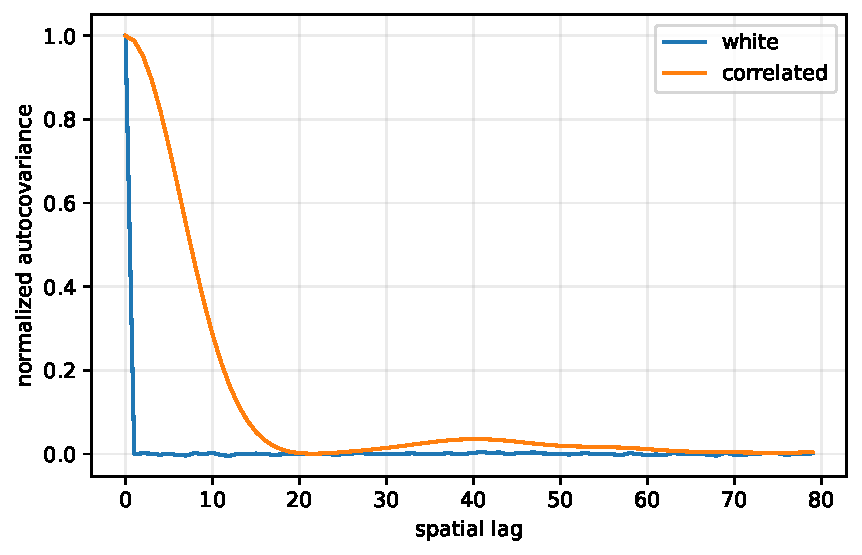
\includegraphics[width=\linewidth]{autocovariance_white_correlated.pdf}
\caption{خودکوواریانس تجربی}
\end{subfigure}
\hfill
\begin{subfigure}{0.48\textwidth}
\centering
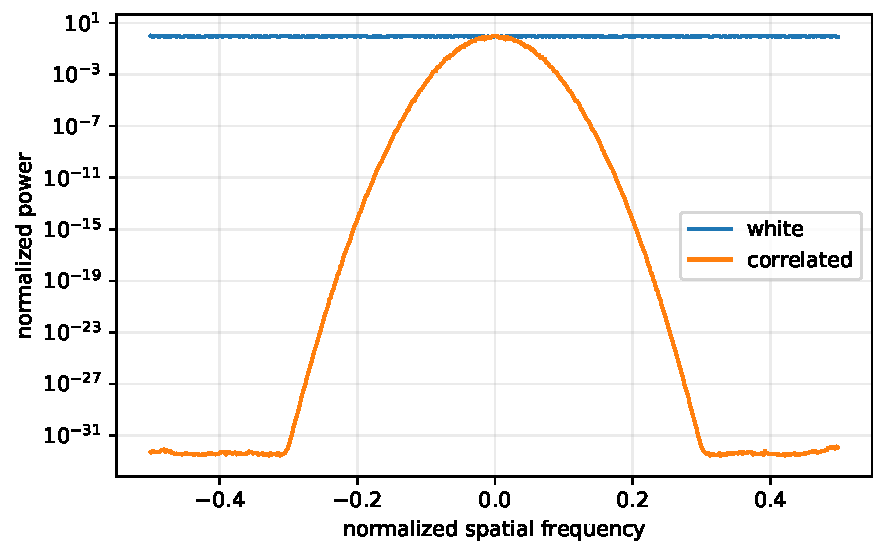
\includegraphics[width=\linewidth]{psd_white_correlated.pdf}
\caption{طیف توان نرمال‌شده}
\end{subfigure}
\caption{مقایسه میدان سفید و میدان هم‌بسته. هموارسازی مکانی طیف را در فرکانس‌های پایین متمرکز می‌کند.}
\label{fig:white-correlated}
\end{figure}

\subsection{دوره‌نگار و محدودیت آن}

برای تحقق محدود \(x[\vect{k}]\) روی شبکه \(M\times N\)، دوره‌نگار
\begin{equation}
\widehat S_{\mathrm{per}}[p,q]
=
\frac{1}{MN}\left|\operatorname{DFT}_2\{x-\bar x\}[p,q]\right|^2
\end{equation}
است. این برآوردگر در حالت کلی واریانس بالایی دارد و با بزرگ‌شدن تصویر لزوماً نقطه‌به‌نقطه پایا نمی‌شود.
میانگین‌گیری روی بلوک‌ها، پنجره‌گذاری و روش \lr{Welch} واریانس را کاهش می‌دهند، ولی تفکیک طیفی را قربانی می‌کنند.

\subsection{واریوگرام}

در زمین‌آمار و تحلیل بافت، نیم‌واریوگرام
\begin{equation}
\gamma(\vect{h})
=
\frac12\E\left[(X(\vect{r}+\vect{h})-X(\vect{r}))^2\right]
\end{equation}
کاربرد دارد. برای میدان \lr{WSS}،
\begin{equation}
\gamma(\vect{h})=C_X(\mathbf{0})-C_X(\vect{h}).
\end{equation}
واریوگرام برای تشخیص برد همبستگی، ناهمسانگردی و نویز مستقل در مبدأ مفید است.

% =============================================================================
\section{فیزیک نویز در زنجیره تصویربرداری}
% =============================================================================

\subsection{نویز شات: چرا پواسون؟}

اگر ورود فوتون‌ها در بازه‌های کوچک تقریباً مستقل و نرخ لحظه‌ای ثابت باشد، تعداد فوتون‌های ثبت‌شده در
زمان نوردهی \(T\) با پارامتر \(\lambda\) مدل می‌شود:
\begin{equation}
N\sim\Poisson(\lambda),
\qquad
\Prob(N=n)=e^{-\lambda}\frac{\lambda^n}{n!}.
\end{equation}
ویژگی بنیادی آن
\begin{equation}
\E[N]=\lambda,
\qquad
\Var(N)=\lambda
\end{equation}
است. بنابراین انحراف معیار \(\sqrt\lambda\) و نسبت سیگنال به نویز شات
\begin{equation}
\SNR_{\mathrm{shot}}=\frac{\lambda}{\sqrt\lambda}=\sqrt\lambda
\end{equation}
است. دو برابر کردن \lr{SNR} شات به چهار برابر فوتون نیاز دارد.

\subsection{نویز خوانش}

نویز تقویت‌کننده، بازنشانی، مدار خوانش و \lr{ADC} اغلب در تقریب نخست با یک مؤلفه گاوسی مستقل از سیگنال
مدل می‌شود:
\begin{equation}
R\sim\Normal(0,\sigma_r^2).
\end{equation}
در نور کم، این مؤلفه می‌تواند بر نویز شات غالب شود. در حسگرهای واقعی، نویز خوانش ممکن است ترکیبی،
دنباله‌سنگین، سطری یا وابسته به کانال باشد.

\subsection{جریان تاریک و نویز تاریک}

حتی بدون نور، الکترون‌های گرمایی تولید می‌شوند. اگر نرخ جریان تاریک \(d\) و زمان نوردهی \(T\) باشد،
مؤلفه تاریک می‌تواند تقریباً \(D\sim\Poisson(dT)\) باشد. میانگین تاریک با کسر فریم تاریک قابل اصلاح است،
اما نوسان شات تاریک باقی می‌ماند. وابستگی شدید جریان تاریک به دما سبب می‌شود کالیبراسیون در دمای متفاوت
قابل انتقال نباشد.

\subsection{ناهمگنی پیکسل: \lr{DSNU} و \lr{PRNU}}

مدل ساده یک پیکسل
\begin{equation}
Y_i=g_i X_i+b_i+\varepsilon_i
\end{equation}
است. تغییرات \(b_i\) میان پیکسل‌ها به ناهمگنی سیگنال تاریک یا \lr{DSNU} و تغییرات \(g_i\) به ناهمگنی
پاسخ نوری یا \lr{PRNU} مربوط است. این مؤلفه‌ها برای یک حسگر ثابت ممکن است تقریباً قطعی باشند، اما در یک
جمعیت حسگر یا با تغییر دما و بهره، پارامترهای تصادفی تلقی می‌شوند.

\subsection{نویز کوانتیزه‌سازی}

اگر کوانتیزه‌سازی یکنواخت با گام \(\Delta\) در ناحیه بدون اشباع انجام شود، در تقریب پُروضوح می‌توان خطا را
مستقل و یکنواخت در نظر گرفت:
\begin{equation}
Q\sim\operatorname{Unif}\left(-\frac\Delta2,\frac\Delta2\right),
\qquad
\Var(Q)=\frac{\Delta^2}{12}.
\end{equation}
این مدل در نزدیکی سطوح کم‌تعداد، اشباع، سیگنال بسیار هموار یا کوانتیزه‌ساز وابسته به سیگنال می‌شکند.

\subsection{پس از \lr{ISP}: نویز دیگر ساده نیست}

دموزاییک کانال‌های رنگ را مخلوط می‌کند، کاهش نویز وابستگی مکانی می‌سازد، شارپ‌سازی طیف نویز را تغییر می‌دهد،
نگاشت تون و گاما نویز را ناهمسان‌واریانس می‌کنند و فشرده‌سازی بلوکی مصنوعات ساختاری می‌افزاید. اگر هدف تخمین
مدل فیزیکی حسگر است، داده \lr{RAW} بر تصویر \lr{sRGB/JPEG} ترجیح دارد.

\begin{researchbox}[استاندارد حسگر]
استاندارد \lr{EMVA 1288} چارچوبی برای اندازه‌گیری و گزارش مشخصه‌هایی مانند بهره تبدیل، بازده کوانتومی،
نویز تاریک، دامنه دینامیکی و نسبت سیگنال به نویز دوربین‌های ماشین‌بینی ارائه می‌کند. در کار پژوهشی، نام استاندارد
به‌تنهایی کافی نیست؛ نسخه، شرایط نور، زمان نوردهی، دما، بهره و نحوه محاسبه باید ثبت شوند \cite{emva1288}.
\end{researchbox}

% =============================================================================
\section{خانواده‌های اصلی مدل نویز}
% =============================================================================

\begin{figure}[H]
\centering
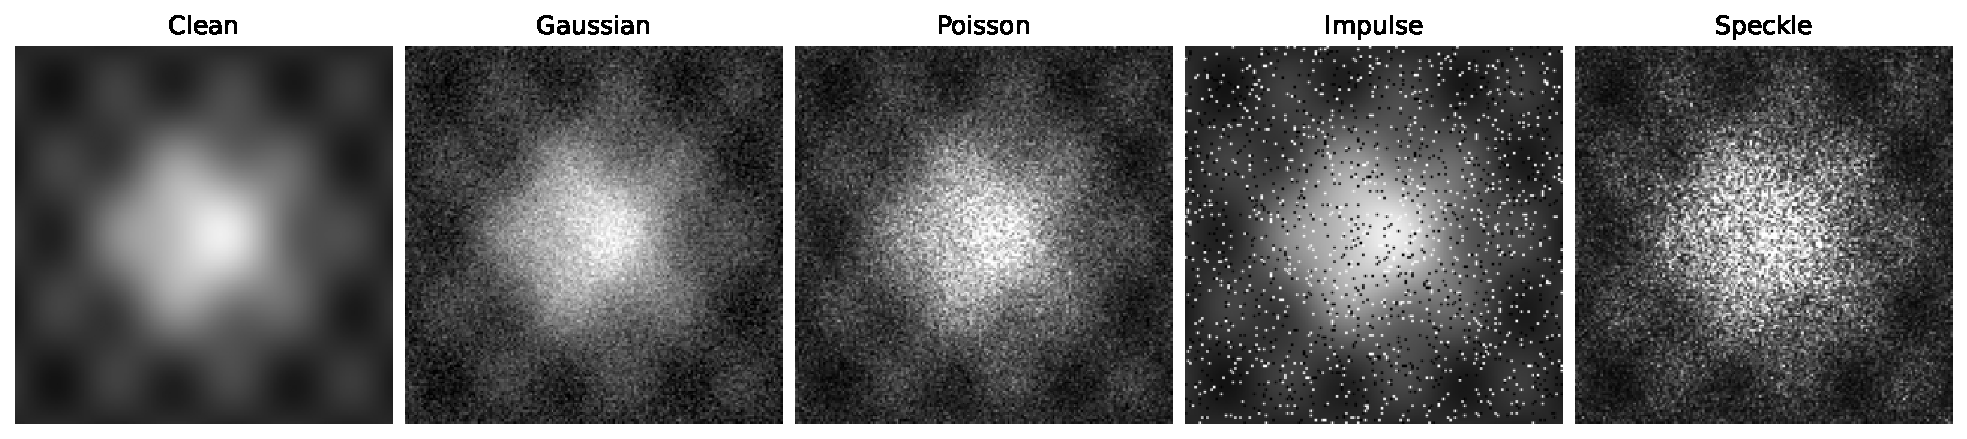
\includegraphics[width=\textwidth]{noise_models_examples.pdf}
\caption{یک تصویر پایه و چهار سازوکار نویز متفاوت. مشابه‌بودن ظاهری به معنای یکسان‌بودن درست‌نمایی نیست.}
\label{fig:noise-models}
\end{figure}

\subsection{نویز گاوسی جمع‌شونده}

مدل
\begin{equation}
Y_i=X_i+N_i,
\qquad
N_i\iid\Normal(0,\sigma^2)
\label{eq:awg}
\end{equation}
دارای درست‌نمایی
\begin{equation}
p(\vect{y}\mid\vect{x},\sigma^2)
=(2\pi\sigma^2)^{-P/2}
\exp\left(-\frac{\norm{\vect{y}-\vect{x}}_2^2}{2\sigma^2}\right)
\end{equation}
است. منفی لگاریتم درست‌نمایی، به‌جز ثابت، همان خطای مربعی است. بنابراین استفاده از \(\ell_2\) یک انتخاب
صرفاً محاسباتی نیست؛ فرض توزیعی مشخصی دارد.

اگر نویز هم‌بسته باشد،
\begin{equation}
\vect{N}\sim\Normal(\mathbf{0},\Sigma),
\end{equation}
و تابع هزینه درست
\begin{equation}
(\vect{y}-\vect{x})\trans\Sigma^{-1}(\vect{y}-\vect{x})
\end{equation}
است، نه خطای مربعی بدون وزن. با تجزیه \(\Sigma=LL\trans\)، سفیدسازی
\(\widetilde{\vect{y}}=L^{-1}\vect{y}\) کوواریانس را به همانی تبدیل می‌کند.

\subsection{نویز پواسون}

برای شمارش فوتون
\begin{equation}
Y_i\mid X_i=x_i\sim\Poisson(\alpha x_i),
\end{equation}
منفی لگاریتم درست‌نمایی، بدون ثابت‌های مستقل از \(x_i\)، برابر است با
\begin{equation}
\mathcal L_{\mathrm P}(\vect{x};\vect{y})
=
\sum_i \left(\alpha x_i-y_i\log(\alpha x_i)\right),
\qquad x_i>0.
\end{equation}
برای پواسون، واریانس تابع سیگنال است و استفاده مستقیم از \(\ell_2\) در شدت‌های بسیار کم می‌تواند وزن‌دهی
نامناسب ایجاد کند.

\subsection{مدل پواسون--گاوسی}

مدل رایج داده خام
\begin{equation}
Y_i=\alpha P_i+G_i,
\qquad
P_i\mid X_i=x_i\sim\Poisson(x_i/\alpha),
\qquad
G_i\sim\Normal(0,\sigma_r^2)
\label{eq:pg}
\end{equation}
است. از قانون واریانس کل،
\begin{align}
\E[Y_i\mid X_i=x_i]&=x_i,\\
\Var(Y_i\mid X_i=x_i)&=\alpha x_i+\sigma_r^2.
\label{eq:mean-variance}
\end{align}
رابطه خطی میان واریانس و میانگین، اساس منحنی انتقال فوتون است.

توزیع دقیق \(Y_i\mid x_i\) کانولوشن پواسون مقیاس‌یافته و گاوسی است:
\begin{equation}
p(y_i\mid x_i)
=
\sum_{k=0}^{\infty}
\frac{e^{-x_i/\alpha}(x_i/\alpha)^k}{k!}
\frac{1}{\sqrt{2\pi\sigma_r^2}}
\exp\left[-\frac{(y_i-\alpha k)^2}{2\sigma_r^2}\right].
\end{equation}
محاسبه مستقیم این مجموع می‌تواند پرهزینه باشد و در شدت بالا تقریب گاوسی ناهمسان‌واریانس به کار می‌رود.

\subsection{نویز ضربه‌ای}

مدل نمک‌وفلفل را می‌توان به شکل آمیخته نوشت:
\begin{equation}
Y_i=
\begin{cases}
X_i,& B_i=0,\\
a,& B_i=1,C_i=0,\\
b,& B_i=1,C_i=1,
\end{cases}
\end{equation}
که \(B_i\sim\Bernoulli(\rho)\) و \(C_i\sim\Bernoulli(\pi)\) است. مدل عمومی‌تر آلودگی
\begin{equation}
p(y_i\mid x_i)=(1-\rho)p_0(y_i\mid x_i)+\rho q(y_i)
\end{equation}
است. در این شرایط، میانگین و مربعات می‌توانند بسیار حساس باشند و برآوردگرهای مقاوم یا مدل آمیخته مناسب‌ترند.

\subsection{نویز اسپکل}

در تصویربرداری همدوس مانند \lr{SAR} و اولتراسوند، مدل ضربی
\begin{equation}
Y_i=X_i S_i
\end{equation}
رایج است. برای میانگین‌گیری \(L\) نگاه مستقل، شدت اسپکل می‌تواند با توزیع گاما مدل شود:
\begin{equation}
S_i\sim\GammaD(L,1/L),
\qquad
\E[S_i]=1,
\qquad
\Var(S_i)=1/L.
\end{equation}
تبدیل لگاریتمی ضرب را به جمع تبدیل می‌کند، ولی نویز لگاریتمی گاوسی دقیق نیست و در شدت نزدیک صفر مسائل عددی دارد.

\subsection{مدل‌های دنباله‌سنگین و مقاوم}

برای نویز با پرت‌های فراوان، توزیع \lr{Student-t}
\begin{equation}
p(r)\propto\left(1+\frac{r^2}{\nu s^2}\right)^{-(\nu+1)/2}
\end{equation}
یا توزیع لاپلاس
\begin{equation}
p(r)=\frac{1}{2b}e^{-|r|/b}
\end{equation}
به‌ترتیب به هزینه‌های لگاریتمی مقاوم و \(\ell_1\) منجر می‌شوند. «مقاوم‌بودن» باید با مدل آلودگی و معیار
خطر تعریف شود، نه صرفاً با انتخاب یک نرم متفاوت.

\subsection{جدول مقایسه مدل‌ها}

\begin{longtable}{p{0.18\textwidth}p{0.25\textwidth}p{0.24\textwidth}p{0.25\textwidth}}
\toprule
\textbf{مدل} & \textbf{رابطه شرطی} & \textbf{ویژگی واریانس} & \textbf{نمونه کاربرد/هشدار}\\
\midrule
\endhead
گاوسی سفید & \(Y=X+N\), \(N\sim\Normal(0,\sigma^2I)\) & ثابت و مستقل از سیگنال & نویز خوانش ساده؛ برای \lr{JPEG} خام‌دستانه است.\\
گاوسی هم‌بسته & \(N\sim\Normal(0,\Sigma)\) & وابستگی مکانی/کانالی & نویز پس از فیلتر، نویز سطری و پردازش داخلی.\\
پواسون & \(Y\mid X\sim\Poisson(\alpha X)\) & متناسب با میانگین & شمارش فوتون؛ در شدت پایین گسسته و نامتقارن.\\
پواسون--گاوسی & \(Y=\alpha P+G\) & \(\alpha X+\sigma_r^2\) & داده خام دوربین؛ پایه \lr{PTC}.\\
ضربه‌ای/آمیخته & \((1-\rho)p_0+\rho q\) & ممکن است نامحدود یا نامعنا شود & پیکسل خراب، خطای انتقال؛ نیازمند روش مقاوم.\\
اسپکل & \(Y=XS\) & متناسب با \(X^2\) & \lr{SAR}/اولتراسوند؛ لگاریتم تقریب را تغییر می‌دهد.\\
کوانتیزه‌سازی & \(Y=Q(X)\) & تقریباً \(\Delta^2/12\) در حالت پُروضوح & در نزدیکی اشباع و بیت کم مستقل نیست.\\
\bottomrule
\end{longtable}

% =============================================================================
\section{استنباط پارامتری: از درست‌نمایی تا کران بنیادی}
% =============================================================================

\subsection{اصل بیشینه درست‌نمایی}

برای داده \(\vect{y}\) و پارامتر \(\theta\)، برآوردگر بیشینه درست‌نمایی
\begin{equation}
\widehat\theta_{\mathrm{ML}}
=\argmax_{\theta}p(\vect{y}\mid\theta)
=\argmin_{\theta}-\log p(\vect{y}\mid\theta)
\end{equation}
است. درست‌نمایی توزیع پارامتر نیست؛ تابعی از پارامتر برای داده ثابت است.

\subsection{مثال: واریانس نویز گاوسی}

اگر \(r_i=y_i-x_i\iid\Normal(0,\sigma^2)\)،
\begin{equation}
\ell(\sigma^2)
=-\frac{n}{2}\log(2\pi\sigma^2)-\frac{1}{2\sigma^2}\sum_i r_i^2.
\end{equation}
با مشتق‌گیری،
\begin{equation}
\widehat\sigma^2_{\mathrm{ML}}=\frac1n\sum_{i=1}^{n}r_i^2.
\end{equation}
اگر میانگین نیز از داده تخمین زده شود، این برآوردگر برای واریانس اریب است و برآوردگر نااریب مخرج \(n-1\) دارد.

\subsection{مثال: نرخ پواسون}

برای \(Y_i\iid\Poisson(\lambda)\)،
\begin{equation}
\ell(\lambda)=-n\lambda+\left(\sum_i y_i\right)\log\lambda-\sum_i\log(y_i!),
\end{equation}
و
\begin{equation}
\widehat\lambda_{\mathrm{ML}}=\bar y.
\end{equation}

\subsection{اطلاعات فیشر}

برای پارامتر اسکالر، اطلاعات فیشر
\begin{equation}
\Fisher(\theta)
=
\E_\theta\left[
\left(\frac{\partial}{\partial\theta}\log p(Y;\theta)\right)^2
\right]
=
-\E_\theta\left[
\frac{\partial^2}{\partial\theta^2}\log p(Y;\theta)
\right]
\end{equation}
است، مشروط بر منظم‌بودن مدل.

\begin{theorem}[کران کرامر--رائو]
اگر \(\widehat\theta\) برآوردگر نااریب و شرایط منظم برقرار باشد،
\begin{equation}
\Var(\widehat\theta)\ge\frac{1}{\Fisher_n(\theta)}.
\end{equation}
برای نمونه‌های مستقل، \(\Fisher_n=n\Fisher_1\).
\end{theorem}

برای یک مشاهده پواسون،
\begin{equation}
\Fisher_1(\lambda)=\frac1\lambda,
\qquad
\Var(\widehat\lambda)\ge\frac{\lambda}{n}.
\end{equation}
میانگین نمونه‌ای این کران را به دست می‌آورد و کارا است.

\subsection{اطلاعات فیشر برای مکان در نویز ناهمسان‌واریانس}

اگر
\begin{equation}
Y_i\sim\Normal(\mu_i(\theta),v_i(\theta)),
\end{equation}
اطلاعات فیشر اسکالر شامل دو مؤلفه است:
\begin{equation}
\Fisher(\theta)
=
\sum_i
\left[
\frac{(\partial_\theta\mu_i)^2}{v_i}
+
\frac12\frac{(\partial_\theta v_i)^2}{v_i^2}
\right].
\end{equation}
پس وابستگی واریانس به پارامتر خود حامل اطلاعات است و نادیده‌گرفتن آن می‌تواند هم برآورد و هم عدم‌قطعیت را مخدوش کند.

\subsection{برآورد بیزی و \lr{MAP}}

با پیشین \(p(\theta)\)، پسین
\begin{equation}
p(\theta\mid\vect{y})
\propto p(\vect{y}\mid\theta)p(\theta)
\end{equation}
و برآورد \lr{MAP}
\begin{equation}
\widehat\theta_{\mathrm{MAP}}
=\argmin_\theta
\left[-\log p(\vect{y}\mid\theta)-\log p(\theta)\right]
\end{equation}
است. منظم‌سازی در بسیاری از مسائل همان منفی لگاریتم پیشین است، ولی این تفسیر تنها وقتی معتبر است که مقیاس و
نرمال‌سازی مدل احتمال نیز سازگار باشند.

% =============================================================================
\section{کالیبراسیون نویز حسگر}
% =============================================================================

\subsection{چرا فریم‌های تکراری لازم‌اند؟}

برای صحنه ثابت و چند ثبت مستقل
\begin{equation}
Y_{i,t}=\mu_i+\varepsilon_{i,t},
\end{equation}
می‌توان میانگین زمانی و واریانس زمانی هر پیکسل را جدا از تغییرات مکانی صحنه تخمین زد. با یک تصویر منفرد،
تفکیک بافت و نویز بدون فرض اضافی ناممکن است.

\subsection{فریم تاریک}

با درپوش بسته و تنظیمات ثابت، چند فریم تاریک ثبت می‌شود. میانگین زمانی تخمینی از الگوی تاریک و واریانس زمانی
تخمینی از نویز خوانش و شات تاریک فراهم می‌کند. برای هر بهره، زمان نوردهی و دما باید کالیبراسیون جداگانه بررسی شود.

\subsection{فریم تخت‌میدان}

یک سطح یکنواخت با چند سطح روشنایی ثبت می‌شود. برای کاهش اثر ناهمگنی ثابت پیکسل، روش تفاضل زوج فریم‌ها مفید است:
\begin{equation}
D=Y^{(1)}-Y^{(2)},
\qquad
\Var(D)=2\Var(Y)
\end{equation}
اگر دو فریم نویز مستقل و میانگین یکسان داشته باشند. بنابراین
\begin{equation}
\widehat{\Var}(Y)=\frac12\widehat{\Var}(D).
\end{equation}

\subsection{منحنی انتقال فوتون}

از مدل \eqref{eq:mean-variance}، در ناحیه خطی و بدون اشباع
\begin{equation}
\Var(Y\mid X=x)=a\,\E[Y\mid X=x]+b.
\label{eq:ptc-line}
\end{equation}
شیب \(a\) به بهره تبدیل و عرض از مبدأ \(b\) به واریانس خوانش در واحد دیجیتال مربوط است. برازش باید روی ناحیه‌ای
انجام شود که پاسخ حسگر خطی است؛ نقاط نزدیک اشباع و ناحیه بسیار تاریک می‌توانند انحراف داشته باشند.

\begin{figure}[H]
\centering
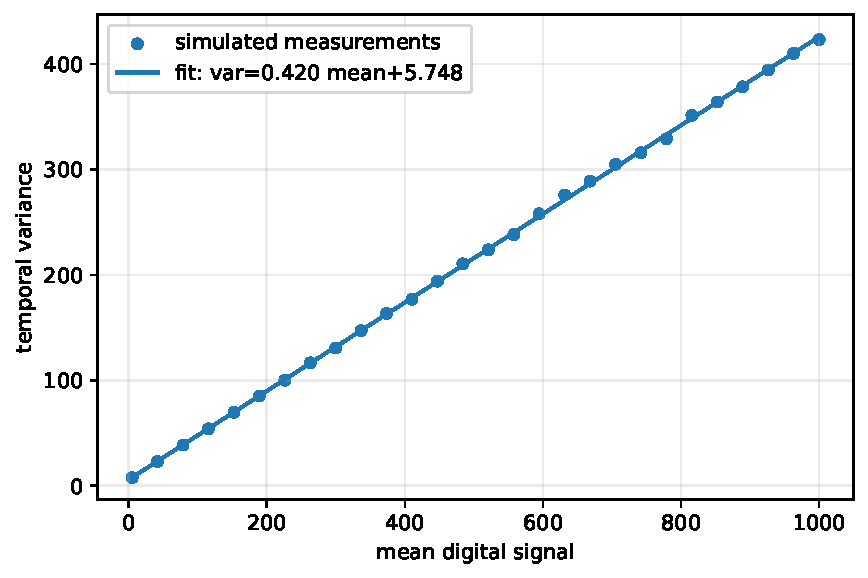
\includegraphics[width=0.72\textwidth]{photon_transfer_curve.pdf}
\caption{نمونه شبیه‌سازی‌شده منحنی انتقال فوتون. نقاط از تفاضل زوج فریم‌ها و خط از برازش \(v=a\mu+b\) به دست آمده‌اند.}
\label{fig:ptc}
\end{figure}

\subsection{برازش وزن‌دار و مقاوم}

واریانس نمونه‌ای در سطح‌های مختلف روشنایی عدم‌قطعیت یکسان ندارد. اگر \(m_j\) تعداد نمونه‌ها در سطح \(j\) باشد،
تقریباً
\begin{equation}
\Var(\widehat v_j)\approx\frac{2v_j^2}{m_j-1}
\end{equation}
برای نویز گاوسی برقرار است. بنابراین برازش وزن‌دار با وزن تقریبی \(w_j\propto(m_j-1)/v_j^2\) منطقی‌تر از کمترین
مربعات بدون وزن است. پیکسل‌های داغ و اشباع نیز باید با روش مقاوم یا قواعد کنترل کیفیت مدیریت شوند.

\subsection{تخمین از یک تصویر: مسئله شناساپذیری}

اگر تنها \(Y=X+N\) مشاهده شود، برای هر تجزیه \(Y=X'+N'\) می‌توان مدل دیگری ساخت. بدون فرض درباره همواری،
تکرارپذیری، استقلال، طیف یا توزیع تصویر پاک، تفکیک سیگنال و نویز شناسا نیست. روش‌های تک‌تصویری ناگزیر از
ساختار محلی، خودشباهتی، شبکه ازپیش‌آموزش‌دیده یا فرض استقلال شرطی استفاده می‌کنند.

\begin{keybox}[اصل کالیبراسیون]
برای اندازه‌گیری نویز حسگر، بهترین داده معمولاً «تصویر طبیعی زیبا» نیست؛ مجموعه‌ای کنترل‌شده از فریم‌های تاریک،
تخت‌میدان، نوردهی‌های مختلف، تکرارهای مستقل و فراداده دقیق است.
\end{keybox}

% =============================================================================
\section{آزمون مدل با تحلیل باقیمانده}
% =============================================================================

اگر مدل میانگین \(\widehat\mu_i\) و واریانس \(\widehat v_i\) باشد، باقیمانده خام و استانداردشده
\begin{equation}
r_i=y_i-\widehat\mu_i,
\qquad
z_i=\frac{r_i}{\sqrt{\widehat v_i}}
\end{equation}
تعریف می‌شوند. یک مدل مناسب باید دست‌کم در داده آزمون مستقل ویژگی‌های زیر را نشان دهد:
\begin{enumerate}
\item \(\E[z_i]\approx0\)؛
\item \(\Var(z_i)\approx1\)؛
\item وابستگی سیستماتیک واریانس به شدت باقی نماند؛
\item خودهمبستگی مکانی و زمانی معنادار کاهش یابد؛
\item شکل توزیع باقیمانده با توزیع فرضی سازگار باشد؛
\item الگوهای سطری، ستونی، رنگی یا بلوکی در نقشه باقیمانده دیده نشود.
\end{enumerate}

\begin{figure}[H]
\centering
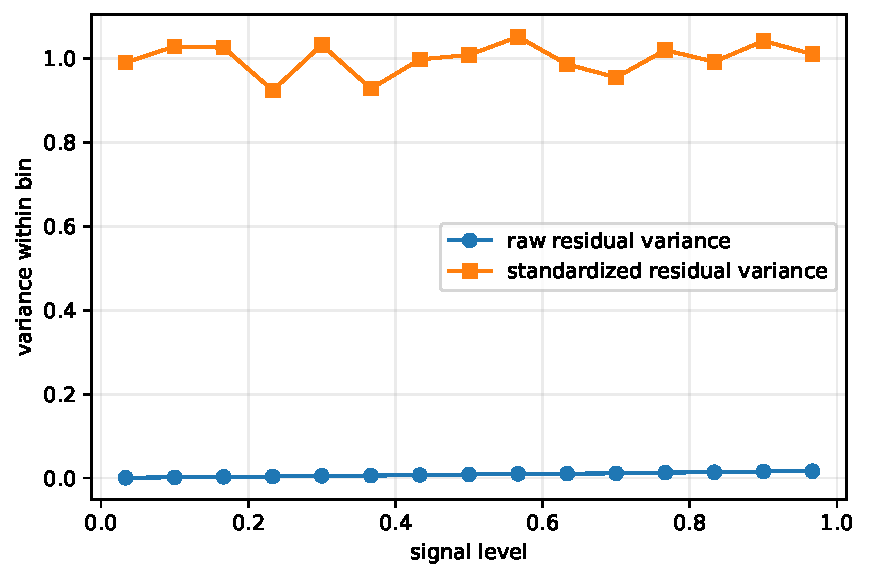
\includegraphics[width=0.72\textwidth]{residual_heteroscedasticity.pdf}
\caption{واریانس باقیمانده خام با شدت تغییر می‌کند، ولی استانداردسازی با مدل صحیح آن را تقریباً ثابت می‌کند.}
\label{fig:residual-hetero}
\end{figure}

\subsection{نمودارهای تشخیصی ضروری}

\begin{enumerate}
\item نمودار باقیمانده در برابر شدت پیش‌بینی‌شده؛
\item نمودار \lr{Q--Q} برای بررسی دنباله‌ها و نامتقارنی؛
\item خودهمبستگی دوبعدی و طیف توان باقیمانده؛
\item نقشه مکانی میانگین و واریانس برای یافتن \lr{DSNU/PRNU}؛
\item هیستوگرام جداگانه برای سطح‌های روشنایی؛
\item تحلیل کانال‌های رنگ و فریم‌های متوالی؛
\item آزمون روی دوربین، \lr{ISO} و نوردهی خارج از داده برازش.
\end{enumerate}

\subsection{مقایسه مدل‌ها}

\lr{AIC} و \lr{BIC} برای مدل‌های پارامتری با درست‌نمایی مشخص به‌ترتیب
\begin{align}
\AIC&=2k-2\ell(\widehat\theta),\\
\BIC&=k\log n-2\ell(\widehat\theta)
\end{align}
هستند. این معیارها جای آزمون خارج از نمونه، تحلیل باقیمانده و بررسی فیزیکی را نمی‌گیرند. مدلی با درست‌نمایی بهتر
اما پارامترهای غیرقابل انتقال یا ناسازگار با حسگر، الزاماً انتخاب مهندسی بهتری نیست.

% =============================================================================
\section{تبدیل‌های تثبیت واریانس}
% =============================================================================

\subsection{روش دلتا}

اگر \(Y\) حول \(\mu\) متمرکز و \(g\) هموار باشد، تقریب تیلور مرتبه اول می‌دهد
\begin{equation}
g(Y)\approx g(\mu)+g'(\mu)(Y-\mu),
\end{equation}
پس
\begin{equation}
\Var(g(Y))\approx[g'(\mu)]^2\Var(Y).
\end{equation}
برای پواسون \(\Var(Y)=\mu\)، با انتخاب \(g'(\mu)\propto\mu^{-1/2}\) به \(g(y)\propto2\sqrt y\) می‌رسیم.

\subsection{تبدیل Anscombe}

تبدیل کلاسیک
\begin{equation}
Z=2\sqrt{Y+\frac38}
\label{eq:anscombe}
\end{equation}
برای داده پواسون و شدت نه‌چندان کم، واریانس را تقریباً واحد و توزیع را تقریباً گاوسی می‌کند. ثابت \(3/8\)
اصلاح بایاس مرتبه بالاتر را بهبود می‌دهد \cite{anscombe1948}.

\begin{figure}[H]
\centering
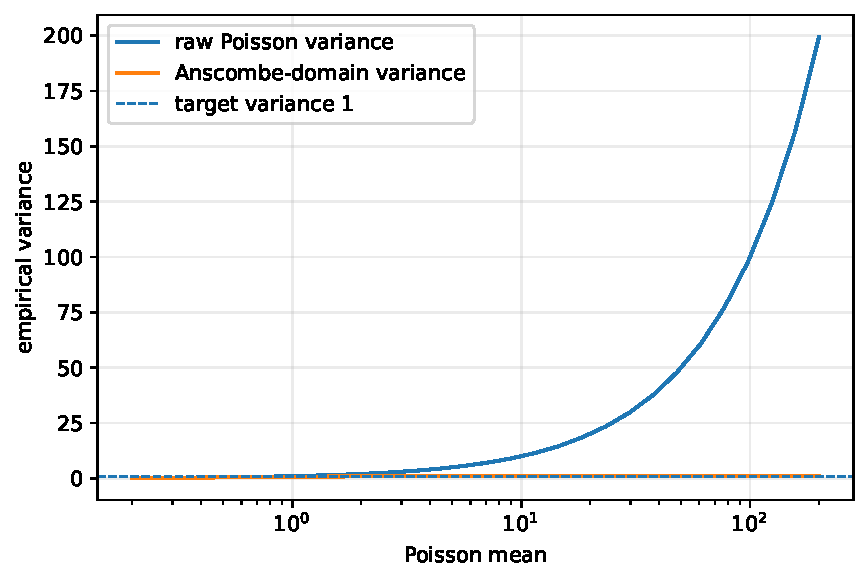
\includegraphics[width=0.72\textwidth]{anscombe_variance.pdf}
\caption{واریانس داده پواسون با میانگین رشد می‌کند، در حالی که واریانس پس از تبدیل Anscombe در گستره وسیعی نزدیک یک است.}
\label{fig:anscombe}
\end{figure}

\subsection{نسخه تعمیم‌یافته برای پواسون--گاوسی}

برای مدل \(Y=\alpha P+G\) با میانگین آفست \(\mu_g\) و واریانس گاوسی \(\sigma_g^2\)، یک شکل رایج تبدیل تعمیم‌یافته
\begin{equation}
Z=\frac{2}{\alpha}
\sqrt{\alpha Y+\frac{3}{8}\alpha^2+\sigma_g^2-\alpha\mu_g}
\end{equation}
است. پارامترگذاری باید با واحدهای مدل سازگار باشد؛ جابه‌جایی میان الکترون، فوتون و کد دیجیتال بدون تبدیل بهره
خطای رایج است \cite{makitalo2013optimal}.

\subsection{مسئله وارون‌سازی}

وارون ساده \(\widehat Y=(Z/2)^2-3/8\) در شدت کم اریب است. پس از حذف نویز در دامنه تبدیل‌شده، باید از وارون
اصلاح‌شده یا برآورد شرطی مناسب استفاده شود. تثبیت واریانس مسئله را دقیقاً به گاوسی سفید تبدیل نمی‌کند؛ فقط تقریب را
در بخشی از دامنه بهبود می‌دهد.

% =============================================================================
\section{از مدل نویز تا یادگیری بدون تصویر پاک}
% =============================================================================

\subsection{Noise2Noise: چرا هدف نویزی می‌تواند کافی باشد؟}

فرض کنید برای یک سیگنال پاک \(X\)، دو مشاهده مستقل شرطی
\begin{equation}
Y=X+N,
\qquad
Y'=X+N',
\qquad
\E[N'\mid X]=0
\end{equation}
داریم. برای تابع \(f\) و زیان مربعی، خطر هدف نویزی
\begin{align}
\E\norm{f(Y)-Y'}_2^2
&=\E\norm{f(Y)-X-N'}_2^2\\
&=\E\norm{f(Y)-X}_2^2+\E\norm{N'}_2^2
-2\E\inner{f(Y)-X}{N'}.
\end{align}
اگر \(N'\) نسبت به \(Y\) به شرط \(X\) مستقل و صفرمیانگین باشد، جمله ضربدری صفر است. بنابراین
\begin{equation}
\argmin_f\E\norm{f(Y)-Y'}^2
=
\argmin_f\E\norm{f(Y)-X}^2.
\label{eq:n2n}
\end{equation}
دو خطر فقط در یک ثابت مستقل از \(f\) تفاوت دارند. این هسته نظری \lr{Noise2Noise} است
\cite{lehtinen2018noise2noise}.

\begin{warningbox}
شرط صفرمیانگین باید نسبت به کمیت هدف و در دامنه‌ای که زیان تعریف شده برقرار باشد. نویز کلیپ‌شده، اشباع،
فشرده‌سازی، misregistration، تغییر حرکت یا پردازش خودکار دوربین می‌تواند این شرط را نقض کند. دو عکس پیاپی
از یک صحنه پویا لزوماً دو مشاهده مستقل از یک \(X\) نیستند.
\end{warningbox}

\subsection{Noise2Self و مفهوم \(\mathcal J\)-ناوردایی}

اندیس‌های تصویر را به زیرمجموعه‌های \(J\) تقسیم کنید. یک نگاشت \(f\) نسبت به \(J\) ناوردا است اگر خروجی روی
مختصات \(J\) به ورودی همان مختصات وابسته نباشد. با فرض استقلال شرطی نویز میان \(J\) و مکمل آن، و
\(\E[Y\mid X]=X\)، می‌توان نشان داد
\begin{equation}
\E\norm{f(Y)-Y}_2^2
=
\E\norm{f(Y)-X}_2^2+\E\norm{Y-X}_2^2
\end{equation}
برای کلاس \(\mathcal J\)-ناوردا. در نتیجه خطای خودنظارتی روی داده نویزی، تا یک ثابت، خطای نسبت به تصویر پاک را
اندازه می‌گیرد \cite{batson2019noise2self}.

\begin{proofbox}[صفرشدن جمله ضربدری]
برای مؤلفه \(i\in J\)، چون \(f_i(Y)\) به \(Y_i\) دسترسی ندارد و نویز \(N_i\) به شرط \(X\) از
\(Y_{J^c}\) مستقل است،
\begin{equation}
\E[(f_i(Y)-X_i)N_i]
=
\E\left[(f_i(Y)-X_i)\E[N_i\mid X,Y_{J^c}]\right]=0.
\end{equation}
جمع روی مختصات هویت خطر را می‌دهد.
\end{proofbox}

\subsection{Noise2Void و شبکه نقطه‌کور}

\lr{Noise2Void} با مخفی‌کردن یا جایگزینی پیکسل هدف مانع کپی مستقیم آن می‌شود و از همبستگی ساختار تصویر با
همسایگی و استقلال نویز استفاده می‌کند \cite{krull2019noise2void}. این روش در نویز مکانی مستقل مناسب‌تر است؛
در نویز نواری، اسپکل هم‌بسته، demosaicing و الگوهای تکراری، همسایه‌ها ممکن است نویز پیکسل هدف را افشا کنند.

\subsection{محدودیت بنیادی خودنظارتی}

اگر نویز هم‌بسته و ساختاری باشد، شبکه می‌تواند همان نویز را پیش‌بینی کند. اگر ساختار سیگنال در مقیاس پیکسل مستقل
باشد، نقطه‌کور بخشی از جزئیات واقعی را نیز حذف می‌کند. پس موفقیت خودنظارتی نه جادو است و نه صرفاً معماری؛ نتیجه
یک شرط استقلال و یک عدم‌تقارن اطلاعاتی طراحی‌شده است.

\begin{futurebox}
مسیر دهه آینده از «یک مدل نویز ثابت برای همه دوربین‌ها» به مدل‌های شرطی بر حسگر، \lr{ISO}، نوردهی، دما، کانال رنگ،
مکان پیکسل و مراحل \lr{ISP} حرکت می‌کند. مدل‌های مولد و diffusion می‌توانند توزیع شرطی پیچیده‌تری بیاموزند، اما
باید با داده خام، کالیبراسیون، آزمون خارج از حسگر و عدم‌قطعیت سنجیده شوند؛ زیبایی خروجی جای درست‌نمایی معتبر را نمی‌گیرد.
\end{futurebox}

% =============================================================================
\section{عدم‌قطعیت، خطر و ارزیابی الگوریتم حذف نویز}
% =============================================================================

\subsection{برآورد نقطه‌ای در برابر توزیع پسین}

برآورد \(\widehat X=f(Y)\) تنها یک نقطه است. در تصویربرداری کم‌نور، چندین تصویر پاک ممکن است با مشاهده سازگار باشند.
توزیع پسین
\begin{equation}
p(\vect{x}\mid\vect{y})
\propto p(\vect{y}\mid\vect{x})p(\vect{x})
\end{equation}
عدم‌قطعیت را حفظ می‌کند. میانگین پسین کمینه‌کننده خطر مربعی، میانه پسین برای زیان قدرمطلق و \lr{MAP} مد توزیع است؛
این سه در توزیع‌های نامتقارن یکسان نیستند.

\subsection{معیارهای دارای مرجع}

برای تصویر پاک \(x\) و بازسازی \(\widehat x\)،
\begin{align}
\MSE&=\frac1P\norm{\widehat x-x}_2^2,\\
\PSNR&=10\log_{10}\frac{L^2}{\MSE},
\end{align}
که \(L\) دامنه بیشینه است. \lr{PSNR} به واحد، گاما، کلیپ و محدوده شدت حساس است. معیارهای ادراکی نیز ممکن است
توهم جزئیات را پاداش دهند. برای کاربرد علمی، خطای پارامتر downstream، کالیبراسیون عدم‌قطعیت و حفظ ساختارهای کم‌کنتراست
باید جداگانه سنجیده شود.

\subsection{ارزیابی بدون مرجع پاک}

وقتی مرجع پاک نداریم، می‌توان از موارد زیر استفاده کرد:
\begin{enumerate}
\item خطر خودنظارتی تحت فرض‌های اثبات‌شده؛
\item دو ثبت مستقل و معیار متقاطع؛
\item تحلیل باقیمانده و سفیدی آن؛
\item آزمون روی phantom یا داده کنترل‌شده؛
\item سازگاری با مدل پیشرو: \(\mathcal H\widehat x\) باید با مشاهده در توزیع نویز سازگار باشد؛
\item عملکرد وظیفه بعدی مانند آشکارسازی، اندازه‌گیری یا قطعه‌بندی؛
\item پایداری نسبت به تغییر حسگر و شدت نویز.
\end{enumerate}

\begin{warningbox}
باقیمانده کاملاً سفید الزاماً نشانه حذف نویز عالی نیست؛ یک روش بیش‌ازحد هموارکننده می‌تواند جزئیات واقعی را نیز در
باقیمانده قرار دهد. باید هم‌زمان ساختار تصویر بازسازی‌شده، سازگاری داده و آزمون‌های وظیفه‌محور بررسی شوند.
\end{warningbox}

% =============================================================================
\section{کارگاه بازتولیدپذیر فصل}
% =============================================================================

\begin{codecontract}
هر شکل عددی فصل باید از یک اسکریپت مشخص ساخته شود؛ بذر تصادفی، پارامتر مدل، تعداد نمونه، واحد شدت و مسیر خروجی
ثبت گردد. فایل تصویری به‌تنهایی نتیجه علمی نیست. همراه هر شکل، داده عددی یا کد تولید آن نگهداری می‌شود.
\end{codecontract}

\subsection{ساخت نویزها با واحدهای روشن}

\noindent\textbf{برنامه ۴.۱: توابع پایه برای نویز گاوسی، پواسون و پواسون--گاوسی}\par
\begin{latin}
\begin{lstlisting}
from __future__ import annotations
import numpy as np
from numpy.typing import NDArray

FloatArray = NDArray[np.float64]

def add_gaussian(
    x: FloatArray,
    sigma: float,
    rng: np.random.Generator,
) -> FloatArray:
    if sigma < 0:
        raise ValueError("sigma must be non-negative")
    return x + rng.normal(0.0, sigma, size=x.shape)


def add_poisson(
    x: FloatArray,
    peak_photons: float,
    rng: np.random.Generator,
) -> FloatArray:
    if peak_photons <= 0:
        raise ValueError("peak_photons must be positive")
    x_nonnegative = np.clip(x, 0.0, None)
    return rng.poisson(peak_photons * x_nonnegative) / peak_photons


def add_poisson_gaussian(
    x: FloatArray,
    gain: float,
    read_sigma: float,
    rng: np.random.Generator,
) -> FloatArray:
    if gain <= 0 or read_sigma < 0:
        raise ValueError("invalid gain or read_sigma")
    photons = rng.poisson(np.clip(x, 0.0, None) / gain)
    return gain * photons + rng.normal(0.0, read_sigma, x.shape)
\end{lstlisting}
\end{latin}

\subsection{تخمین منحنی میانگین--واریانس}

\noindent\textbf{برنامه ۴.۲: برازش ساده مدل واریانس خطی؛ در پروژه نهایی باید وزن‌دار و مقاوم شود}\par
\begin{latin}
\begin{lstlisting}
import numpy as np


def fit_mean_variance(means: np.ndarray,
                      variances: np.ndarray) -> tuple[float, float]:
    means = np.asarray(means, dtype=float)
    variances = np.asarray(variances, dtype=float)
    valid = np.isfinite(means) & np.isfinite(variances) & (variances >= 0)
    if valid.sum() < 3:
        raise ValueError("at least three valid levels are required")
    A = np.column_stack([means[valid], np.ones(valid.sum())])
    slope, intercept = np.linalg.lstsq(A, variances[valid], rcond=None)[0]
    return float(slope), float(intercept)
\end{lstlisting}
\end{latin}

\subsection{آزمون سفیدی باقیمانده}

برای باقیمانده دوبعدی \(r\)، می‌توان خودهمبستگی نرمال‌شده را با \lr{FFT} محاسبه کرد:
\noindent\textbf{برنامه ۴.۳: خودهمبستگی دوبعدی نرمال‌شده}\par
\begin{latin}
\begin{lstlisting}
import numpy as np


def normalized_acf2(residual: np.ndarray) -> np.ndarray:
    r = np.asarray(residual, dtype=float)
    r = r - np.mean(r)
    spectrum = np.fft.fft2(r)
    acf = np.fft.ifft2(np.abs(spectrum) ** 2).real
    acf = np.fft.fftshift(acf)
    center = tuple(s // 2 for s in acf.shape)
    denom = acf[center]
    if denom <= 0:
        raise ValueError("residual variance must be positive")
    return acf / denom
\end{lstlisting}
\end{latin}

\begin{workshopbox}[آزمایش مرکزی فصل]
یک تصویر تخت‌میدان مصنوعی در ۲۰ سطح روشنایی بسازید. در هر سطح ۳۰ فریم پواسون--گاوسی تولید کنید.
سپس:
\begin{enumerate}
\item واریانس را هم از فریم‌ها و هم از تفاضل زوج‌ها تخمین بزنید؛
\item مدل \(v=a\mu+b\) را با کمترین مربعات، کمترین مربعات وزن‌دار و \lr{Huber} برازش کنید؛
\item ۱ درصد پیکسل داغ اضافه کنید و تغییر پارامترها را گزارش دهید؛
\item باقیمانده استانداردشده را از نظر واریانس، \lr{Q--Q} و خودهمبستگی بررسی کنید؛
\item اثر حذف نقاط نزدیک اشباع را تحلیل کنید؛
\item بازه اطمینان پارامترها را با bootstrap سطح روشنایی محاسبه کنید.
\end{enumerate}
\end{workshopbox}

\subsection{پرامپت کنترل‌شده برای Codex}

\begin{tcolorbox}[colback=CodeGray,colframe=DeepBlue,title={پرامپت پیشنهادی اجرای آزمایش فصل},breakable]
\begin{latin}
Create a reproducible Python package for Chapter 4 of a graduate image-processing course.
Implement Gaussian, Poisson, Poisson--Gaussian, impulse, speckle, row-correlated, and quantization noise.
Use NumPy, SciPy, Matplotlib, pandas, pytest, and type hints. Generate controlled dark-frame and flat-field
experiments, pair-difference photon-transfer curves, weighted and robust mean--variance fitting, Fisher-information
checks, Anscombe variance-stabilization plots, and residual diagnostics in space and frequency. Save every numeric
result to CSV and every figure to both PDF and PNG. Use a fixed seed from a configuration file. Add unit tests for
mean/variance identities, covariance positive-semidefiniteness, the Wiener--Khinchin numerical relation, and the
Noise2Noise risk identity by Monte Carlo. Never fabricate outputs; fail loudly if an expected file is missing.
Include README instructions for Windows PowerShell and Linux/macOS.
\end{latin}
\end{tcolorbox}

% =============================================================================
\section{تمرین‌های ریاضی، محاسباتی و پژوهشی}
% =============================================================================

\subsection*{تمرین‌های مفهومی و اثباتی}
\begin{enumerate}
\item نشان دهید ماتریس کوواریانس هر بردار تصادفی متقارن و نیمه‌مثبت معین است. عکس این گزاره را نیز برای ساخت یک بردار گاوسی بیان کنید.
\item مثالی از یک فرایند ایستای وسیع ولی غیرگاوسی ارائه کنید که ایستایی سخت آن از اطلاعات مرتبه دوم قابل نتیجه‌گیری نباشد.
\item ثابت کنید عبور نویز سفید با واریانس \(\sigma^2\) از فیلتر \(h\)، واریانس خروجی \(\sigma^2\norm h_2^2\) ایجاد می‌کند.
\item رابطه واریوگرام و کوواریانس را برای میدان \lr{WSS} استخراج کنید.
\item برای \(Y\sim\Poisson(\lambda)\)، اطلاعات فیشر و کران کرامر--رائو را محاسبه کنید.
\item برای مدل \(Y=X+N\) با \(N\sim\operatorname{Laplace}(0,b)\)، نشان دهید \lr{MLE} برای \(X\) ثابت، میانه نمونه است.
\item خطر \lr{Noise2Noise} را برای زیان قدرمطلق تحلیل کنید. هدف به کدام کمیت شرطی همگرا می‌شود؟
\item در اثبات \lr{Noise2Self} دقیقاً مشخص کنید کدام شرط استقلال برای صفرشدن جمله ضربدری لازم است.
\item با روش دلتا تبدیل تثبیت واریانس برای مدلی با \(\Var(Y\mid X=x)=ax^2+b\) را به‌طور ضمنی استخراج کنید.
\item نشان دهید سفیدسازی با \(L^{-1}\) در صورت \(\Sigma=LL\trans\) کوواریانس همانی ایجاد می‌کند.
\end{enumerate}

\subsection*{تمرین‌های محاسباتی}
\begin{enumerate}
\item برای پنج سطح شدت، ۱۰ هزار نمونه پواسون تولید و میانگین، واریانس، skewness و خطای تقریب گاوسی را رسم کنید.
\item دوره‌نگار یک نویز سفید، نویز هموارشده، نویز سطری و مصنوعات بلوکی \lr{JPEG} را مقایسه کنید.
\item ماتریس کوواریانس وصله‌های \(8\times8\) را تخمین بزنید و مقادیر ویژه آن را برای تصویر طبیعی و نویز سفید مقایسه کنید.
\item منحنی انتقال فوتون را با و بدون تفاضل زوج‌ها بسازید و اثر \lr{PRNU} را توضیح دهید.
\item تبدیل Anscombe را در شدت‌های کمتر از یک فوتون بررسی و بایاس وارون ساده را اندازه‌گیری کنید.
\item یک مدل نویز اشتباه را عمداً برازش دهید و نشان دهید تحلیل باقیمانده چگونه خطا را آشکار می‌کند.
\item نویز هم‌بسته بسازید و تفاوت کمترین مربعات معمولی و کمترین مربعات تعمیم‌یافته را بسنجید.
\item یک شبکه نقطه‌کور کوچک را روی نویز مستقل و نویز سطری آموزش دهید و شکست شرط استقلال را مستند کنید.
\end{enumerate}

\subsection*{تمرین‌های پژوهشی}
\begin{enumerate}
\item یک دوربین یا گوشی انتخاب و بررسی کنید آیا خروجی \lr{RAW} در دسترس است. پروتکل ثبت فریم تاریک و تخت‌میدان طراحی کنید.
\item سه مقاله جدید حذف نویز واقعی را انتخاب و مشخص کنید هر مقاله نویز را در کدام دامنه، با چه داده و چه فرضی مدل کرده است.
\item یک جدول «ادعا ـ فرض ـ آزمون» برای یک مقاله self-supervised denoising بسازید.
\item بررسی کنید آیا معیارهای ادراکی در یک کاربرد پزشکی یا نجومی می‌توانند جزئیات ساختگی را پاداش دهند.
\item یک پروتکل انتقال بین حسگرها طراحی کنید که آموزش روی یک دوربین و آزمون روی دوربین دیگر را شامل شود.
\end{enumerate}

% =============================================================================
\section{تقسیم پیشنهادی فصل به ویدئوهای ۱۵ دقیقه‌ای}
% =============================================================================

\begin{videobox}
\begin{enumerate}
\item \textbf{ویدئو ۱:} نویز به‌عنوان بخشی از اندازه‌گیری؛ تفاوت تحقق و توزیع.
\item \textbf{ویدئو ۲:} تصویر به‌صورت بردار و میدان تصادفی؛ توزیع‌های متناهی‌بعدی.
\item \textbf{ویدئو ۳:} میانگین، کوواریانس و نیمه‌مثبت‌بودن؛ مثال عددی.
\item \textbf{ویدئو ۴:} ایستایی سخت، \lr{WSS}، همسانگردی و ارگودیسیته.
\item \textbf{ویدئو ۵:} سفیدی، استقلال و مثال نامرتبط ولی وابسته.
\item \textbf{ویدئو ۶:} قضیه وینر--خینچین، طیف توان و دوره‌نگار.
\item \textbf{ویدئو ۷:} فیزیک حسگر: فوتون، خوانش، تاریک، \lr{DSNU/PRNU}.
\item \textbf{ویدئو ۸:} مدل‌های گاوسی، پواسون و پواسون--گاوسی.
\item \textbf{ویدئو ۹:} نویز ضربه‌ای، اسپکل، هم‌بسته و دنباله‌سنگین.
\item \textbf{ویدئو ۱۰:} \lr{MLE}، اطلاعات فیشر و کران کرامر--رائو.
\item \textbf{ویدئو ۱۱:} فریم تاریک، تخت‌میدان و منحنی انتقال فوتون.
\item \textbf{ویدئو ۱۲:} تحلیل باقیمانده و تشخیص مدل اشتباه.
\item \textbf{ویدئو ۱۳:} روش دلتا، Anscombe و مسئله وارون‌سازی.
\item \textbf{ویدئو ۱۴:} اثبات Noise2Noise و نقش صفرمیانگین.
\item \textbf{ویدئو ۱۵:} Noise2Self/Noise2Void و شکست در نویز هم‌بسته.
\item \textbf{ویدئو ۱۶:} کارگاه نهایی، گزارش علمی و مسیر اتصال به فصل پنجم.
\end{enumerate}
\end{videobox}

% =============================================================================
\section{جمع‌بندی و پل به فصل پنجم}
% =============================================================================

\begin{summarybox}
\begin{enumerate}
\item تصویر تصادفی یک تحقق از یک بردار یا میدان تصادفی است؛ هیستوگرام به‌تنهایی ساختار مکانی را توصیف نمی‌کند.
\item کوواریانس و طیف توان دو نمایش فوریه‌ای از وابستگی مرتبه دوم‌اند.
\item نویز سفید، مستقل و گاوسی سه مفهوم متفاوت‌اند؛ فقط در حالت گاوسی نامرتبط‌بودن به استقلال منجر می‌شود.
\item نویز شات از شمارش فوتون می‌آید و واریانس آن با میانگین رشد می‌کند؛ نویز خوانش در تقریب نخست مستقل از سیگنال است.
\item مدل پواسون--گاوسی رابطه \(v=a\mu+b\) را ایجاد می‌کند و پایه کالیبراسیون حسگر است.
\item انتخاب هزینه \(\ell_2\)، \(\ell_1\) یا هزینه پواسون باید از درست‌نمایی و هدف خطر ناشی شود.
\item هیچ مدل نویزی بدون تحلیل باقیمانده، آزمون خارج از نمونه و بررسی فیزیکی کامل نیست.
\item تثبیت واریانس و یادگیری خودنظارتی ابزارهایی مبتنی بر فرض‌اند، نه راه‌های حذف نیاز به مدل‌سازی.
\item در فصل پنجم، همین مدل‌های نویز وارد طراحی فیلتر و بازسازی می‌شوند: وینر، تیکانوف، تغییرات کلی، روش‌های پروگزیمال،
\lr{plug-and-play} و شبکه‌های بازشده همگی به یک مدل داده و یک پیشین نیاز دارند.
\end{enumerate}
\end{summarybox}

\backmatter
\chapter*{منابع منتخب فصل}
\addcontentsline{toc}{chapter}{منابع منتخب فصل}

\begin{latin}
\begin{thebibliography}{99}

\bibitem{papoulis}
A. Papoulis and S. U. Pillai,
\textit{Probability, Random Variables, and Stochastic Processes},
4th ed., McGraw--Hill, 2002.

\bibitem{goodman}
J. W. Goodman,
\textit{Statistical Optics},
2nd ed., Wiley, 2015.

\bibitem{gonzalez}
R. C. Gonzalez and R. E. Woods,
\textit{Digital Image Processing},
4th ed., Pearson, 2018.

\bibitem{kay}
S. M. Kay,
\textit{Fundamentals of Statistical Signal Processing: Estimation Theory},
Prentice Hall, 1993.

\bibitem{vanTrees}
H. L. Van Trees,
\textit{Detection, Estimation, and Modulation Theory, Part I},
2nd ed., Wiley, 2001.

\bibitem{emva1288}
European Machine Vision Association,
\textit{EMVA 1288: Standard for Characterization and Presentation of Specification Data for Image Sensors and Cameras},
Release 4.0, 2021.

\bibitem{healey1994radiometric}
G. E. Healey and R. Kondepudy,
``Radiometric CCD camera calibration and noise estimation,''
\textit{IEEE Transactions on Pattern Analysis and Machine Intelligence},
vol. 16, no. 3, pp. 267--276, 1994.

\bibitem{foi2008practical}
A. Foi, M. Trimeche, V. Katkovnik, and K. Egiazarian,
``Practical Poissonian--Gaussian noise modeling and fitting for single-image raw-data,''
\textit{IEEE Transactions on Image Processing},
vol. 17, no. 10, pp. 1737--1754, 2008.

\bibitem{anscombe1948}
F. J. Anscombe,
``The transformation of Poisson, binomial and negative-binomial data,''
\textit{Biometrika}, vol. 35, nos. 3--4, pp. 246--254, 1948.

\bibitem{makitalo2013optimal}
M. Mäkitalo and A. Foi,
``Optimal inversion of the generalized Anscombe transformation for Poisson--Gaussian noise,''
\textit{IEEE Transactions on Image Processing},
vol. 22, no. 1, pp. 91--103, 2013.

\bibitem{lehtinen2018noise2noise}
J. Lehtinen, J. Munkberg, J. Hasselgren, S. Laine, T. Karras, M. Aittala, and T. Aila,
``Noise2Noise: Learning image restoration without clean data,''
in \textit{Proceedings of ICML}, pp. 2965--2974, 2018.

\bibitem{krull2019noise2void}
A. Krull, T.-O. Buchholz, and F. Jug,
``Noise2Void: Learning denoising from single noisy images,''
in \textit{Proceedings of CVPR}, pp. 2129--2137, 2019.

\bibitem{batson2019noise2self}
J. Batson and L. Royer,
``Noise2Self: Blind denoising by self-supervision,''
in \textit{Proceedings of ICML}, pp. 524--533, 2019.

\bibitem{abdelhamed2018sidd}
A. Abdelhamed, S. Lin, and M. S. Brown,
``A high-quality denoising dataset for smartphone cameras,''
in \textit{Proceedings of CVPR}, pp. 1692--1700, 2018.

\bibitem{plotz2017benchmarking}
T. Plötz and S. Roth,
``Benchmarking denoising algorithms with real photographs,''
in \textit{Proceedings of CVPR}, pp. 1586--1595, 2017.

\bibitem{brooks2019unprocessing}
T. Brooks, B. Mildenhall, T. Xue, J. Chen, D. Sharlet, and J. T. Barron,
``Unprocessing images for learned raw denoising,''
in \textit{Proceedings of CVPR}, pp. 11036--11045, 2019.

\end{thebibliography}
\end{latin}

\chapter*{راهنمای کامپایل و کنترل فونت}
\addcontentsline{toc}{chapter}{راهنمای کامپایل و کنترل فونت}

این فایل باید با \lr{XeLaTeX} کامپایل شود. در \lr{TeXstudio} از مسیر
\lr{Options > Configure TeXstudio > Build} کامپایلر پیش‌فرض را روی \lr{XeLaTeX} قرار دهید.
دو بار کامپایل برای تکمیل فهرست مطالب لازم است.

فونت اصلی همان \lr{Amiri} مورد استفاده فصل‌های دوم و سوم است. اگر روی سامانه نصب نباشد، فایل به‌طور خودکار
به \lr{Noto Naskh Arabic} برمی‌گردد. فونت لاتین و کد نیز به‌ترتیب \lr{DejaVu Serif} و
\lr{DejaVu Sans Mono} هستند و برای آن‌ها نیز جایگزین خودکار تعریف شده است. هیچ فایل فونتی همراه بسته توزیع نشده است.

\end{document}
